\documentclass[11pt]{article}
\usepackage{icmlko}
\begin{document}

\title{같은 실험이 4/11 도 되고 7/11 도 된다 --- 내 자에 눈금을 판다}
\author{월드모델 실험실}
\date{노트 434 · 2026년 8월 5일}
\maketitle

\begin{abstract}
노트 433이 스스로 ``제일 약한 곳''이라 적었다 --- \emph{LODO 는 씨앗 셋인데
내가 부호로 세는 차가 $\pm 0.01$ 대다.} 그 자를 쟀다.

\begin{center}
\begin{tabular}{lr}
\hline
LODO 수준의 씨앗 묶음 SD & $0.0069$ (최대 $0.0124$) \\
\textbf{짝 차이의 묶음 간 SD} & $\mathbf{0.0036}$ \\
\hline
부호가 두 묶음에서 같은 도메인 & $6/11$ \\
\textbf{깊이 12 가 이긴 도메인} & \textbf{묶음A $4/11$ · 묶음B $7/11$} \\
\hline
\end{tabular}
\end{center}

\textbf{같은 실험이 씨앗만 바꾸면 $4/11$ 도 되고 $7/11$ 도 된다.} 규약의
기각 문턱이 $\le 3$ 이고 채택 문턱이 $\ge 8$ 이니, \textbf{그 한 번의 셈이
기각 근처에서 채택 근처까지 오간다.} 노트 431·432·433이 인용한 셈들은
\textbf{이 자로는 그만한 정밀도가 없었다.}

짝짓기가 잡음을 절반으로 줄이긴 한다($0.0069 \to 0.0036$). 모자랐을 뿐이다.
\end{abstract}

\section{자에 눈금을 판다}

뒤집힌 넷은 전부 $|\Delta| < 0.01$ 이고, 안 뒤집힌 것 중 큰 것들
(아이돌 $-0.027/-0.025$ · 팝업 $-0.026/-0.026$)은 소수점 셋째 자리까지 맞는다.
\textbf{부호는 차가 잡음을 넘을 때만 뜻이 있다.}

\begin{center}
\textbf{LODO 다수결은 $|\Delta| > 3 \times$ 짝 잡음($0.0108$)인 도메인만
센다.}
\end{center}

\section{문턱을 달고 세 판정을 다시 읽는다}

\begin{center}
\begin{tabular}{lll}
\hline
 & 문턱 넘는 도메인 & 읽기 \\
\hline
깊이 $12$ & $\mathbf{2/11}$ --- 아이돌 $-0.026$ · 팝업 $-0.026$ &
\textbf{둘 다 음수} \\
\texttt{grp} & $7/11$ --- 양수 4 · 음수 3 & \textbf{정말 반반} \\
$K{=}64$ & $0/11$ & 셈이 무의미 \\
\hline
\end{tabular}
\end{center}

\textbf{판정은 셋 다 그대로 선다.} 다만 근거가 달라진다.

\begin{itemize}
\item \textbf{깊이 12 되돌림}(노트 432) --- $4/11$ 이라는 셈이 아니라
\textbf{잴 수 있는 두 도메인이 둘 다 음수}라는 것이 근거다. 오히려 전보다
낫다.
\item \textbf{grp 일반화 미성립}(노트 433) --- 문턱을 넘는 일곱 중 넷 대 셋.
\textbf{반반이라는 결론이 더 또렷해졌다.}
\item \textbf{$K{=}64$ 기각}(노트 431) --- LODO 셈은 아무 말도 못 한다.
그 판정은 \textbf{판이 포화라 한 것}에 기대고, 그건 그대로다.
\end{itemize}

\section{내가 틀린 것은 결론이 아니라 정밀도다}

노트 431이 ``한 짝의 $1.000$ 이 열한 짝에서 $3/11$ 이 된다''고 적으며 한 짝의
좁은 구간을 나무랐다. 옳았다. 그런데 \textbf{그 자리에서 내가 든 열한 짝짜리
자도 눈금이 굵었다} --- 그 노트의 $3/11$ 은 지금 보면 문턱을 넘는 도메인이
하나도 없는 셈이었다.

\textbf{자를 바꿀 때는 새 자의 잡음도 같이 재야 한다.} 노트 430에서 LODO 를
지을 때 씨앗 잡음을 안 쟀고, 노트 433에서 스스로 적어 두고도 세 노트를 더
쓴 뒤에야 쟀다.

\begin{tabular}{lp{7.0cm}}
\hline
씨앗을 늘린다 & 문턱을 넘는 도메인이 깊이에서 둘뿐이다. 씨앗 셋 $\to$ 아홉이면
잡음이 $\sqrt{3}$ 배 줄어 문턱이 $0.006$ 이 된다 \\
규약에 단서 & LODO 다수결에 \textbf{잡음 문턱}을 박아 넣는다 \\
집 안팎 & 노트 433의 물음은 그대로다 --- 다만 이제 그것도 문턱을 넘는
도메인으로만 물어야 한다 \\
\hline
\end{tabular}

\begin{figure}[h]
\centering
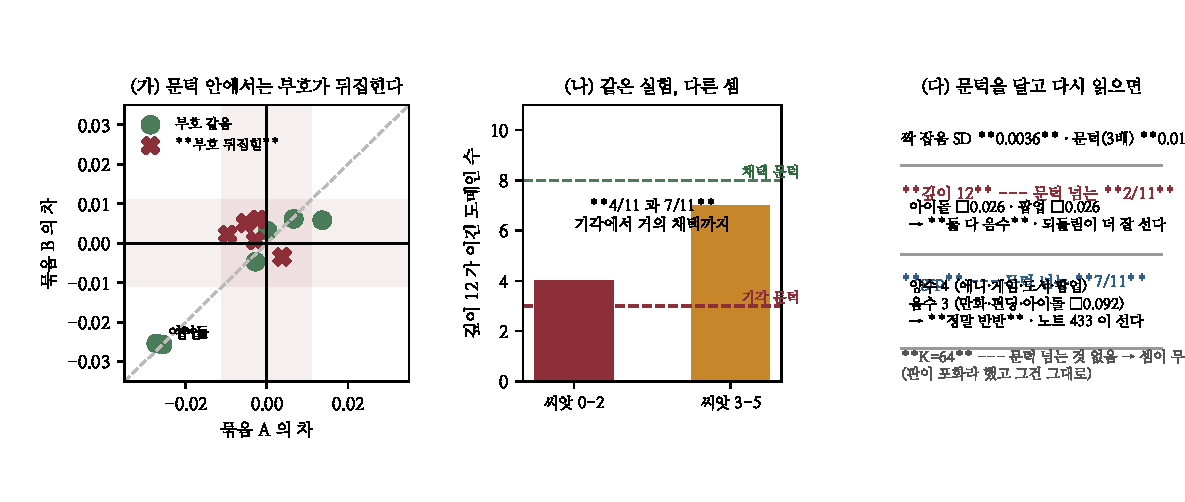
\includegraphics[width=\textwidth]{figs/fig434.pdf}
\caption{(가) 문턱 안(붉은 띠)에서는 부호가 뒤집힌다. (나) 같은 실험이
$4/11$ 과 $7/11$. (다) 문턱을 달고 다시 읽은 세 판정.}
\end{figure}

\end{document}
